\chapter{Introduction}

Hardware components have been known to be extremely complex due to
concurrency. A system having concurrency implies that independent
works can be done simultaneously, and it usually occurs as a name of
optimization. For example, instruction pipelining is one of
representative optimizations, which employes an instruction-level
parallelism to handle multiple executions at the same time.

Modularity has been considered as an effective way to design and
understand such complex hardware components. Modularity indicates that
a complex hardware can be constructed by composing simple
modules. Several Hardware Description Languages (HDLs) such as Verilog
employ the notion of modules, each of which acts as a simple unit
component.

Among various HDLs, \Bluespec{}~\cite{bsdef, bsref} allows to design
hardware based not only on modularity, but also the prevalent paradigm
called Guarded Atomic Actions (GAAs). Even though a certain language
allows to design hardware in a modular manner, modules cannot be
independently designed if they are entangled with clock-timing
issues. For instance, when two modules are connected with wires and
one module becomes to need shorter clock cycles by optimization, the
other module should follow that cycle, or the optimized module should
maintain the original clock even if it is optimized.

Following the concepts of modularity and GAA, we have been defining a
framework called \Kami{}, which is for specifying, verifying, and
synthesizing \Bluespec{}-style hardware components. \Kami{} presents a
domain specific language similar to Bluespec, and aims to prove the
correctness of hardware automatically. In order for correctness proof,
we also have defined formal semantics of the \Kami{} language, which
is based on the modularity concept. The framework has been built on
the Coq proof assistant.

Modularity fits for scalable verification, especially with theorem
provers. In terms of verification, modularity implies that complex
hardware components can be verified if each simple element is
verified. And in many cases, we reuse such simple components for
different uses. From the perspective of theorem proving, reusing a
hardware component indicates that we can also reuse its correctness
proof. Thanks to the modular semantics in \Kami{}, it is indeed
possible to use the proof of a component whenever it is used for the
part of a design.

An important aspect of the modular semantics is that modules
communicate by labels. It is originated from the concept called
Labeled Transition System (LTS). Each module changes its internal
state and the corresponding label is generated during the state
transition. On the modular semantics, labels are method calls. In
other words, modules communicate by calling methods of target modules.
The modular semantics also take advantage of the LTS concept to define
behaviors of \emph{open systems}. Open systems have external
interactions, which cannot be figured out unless it is connected with
some other modules which can respond to them.

\begin{figure}[t]
  \centering
  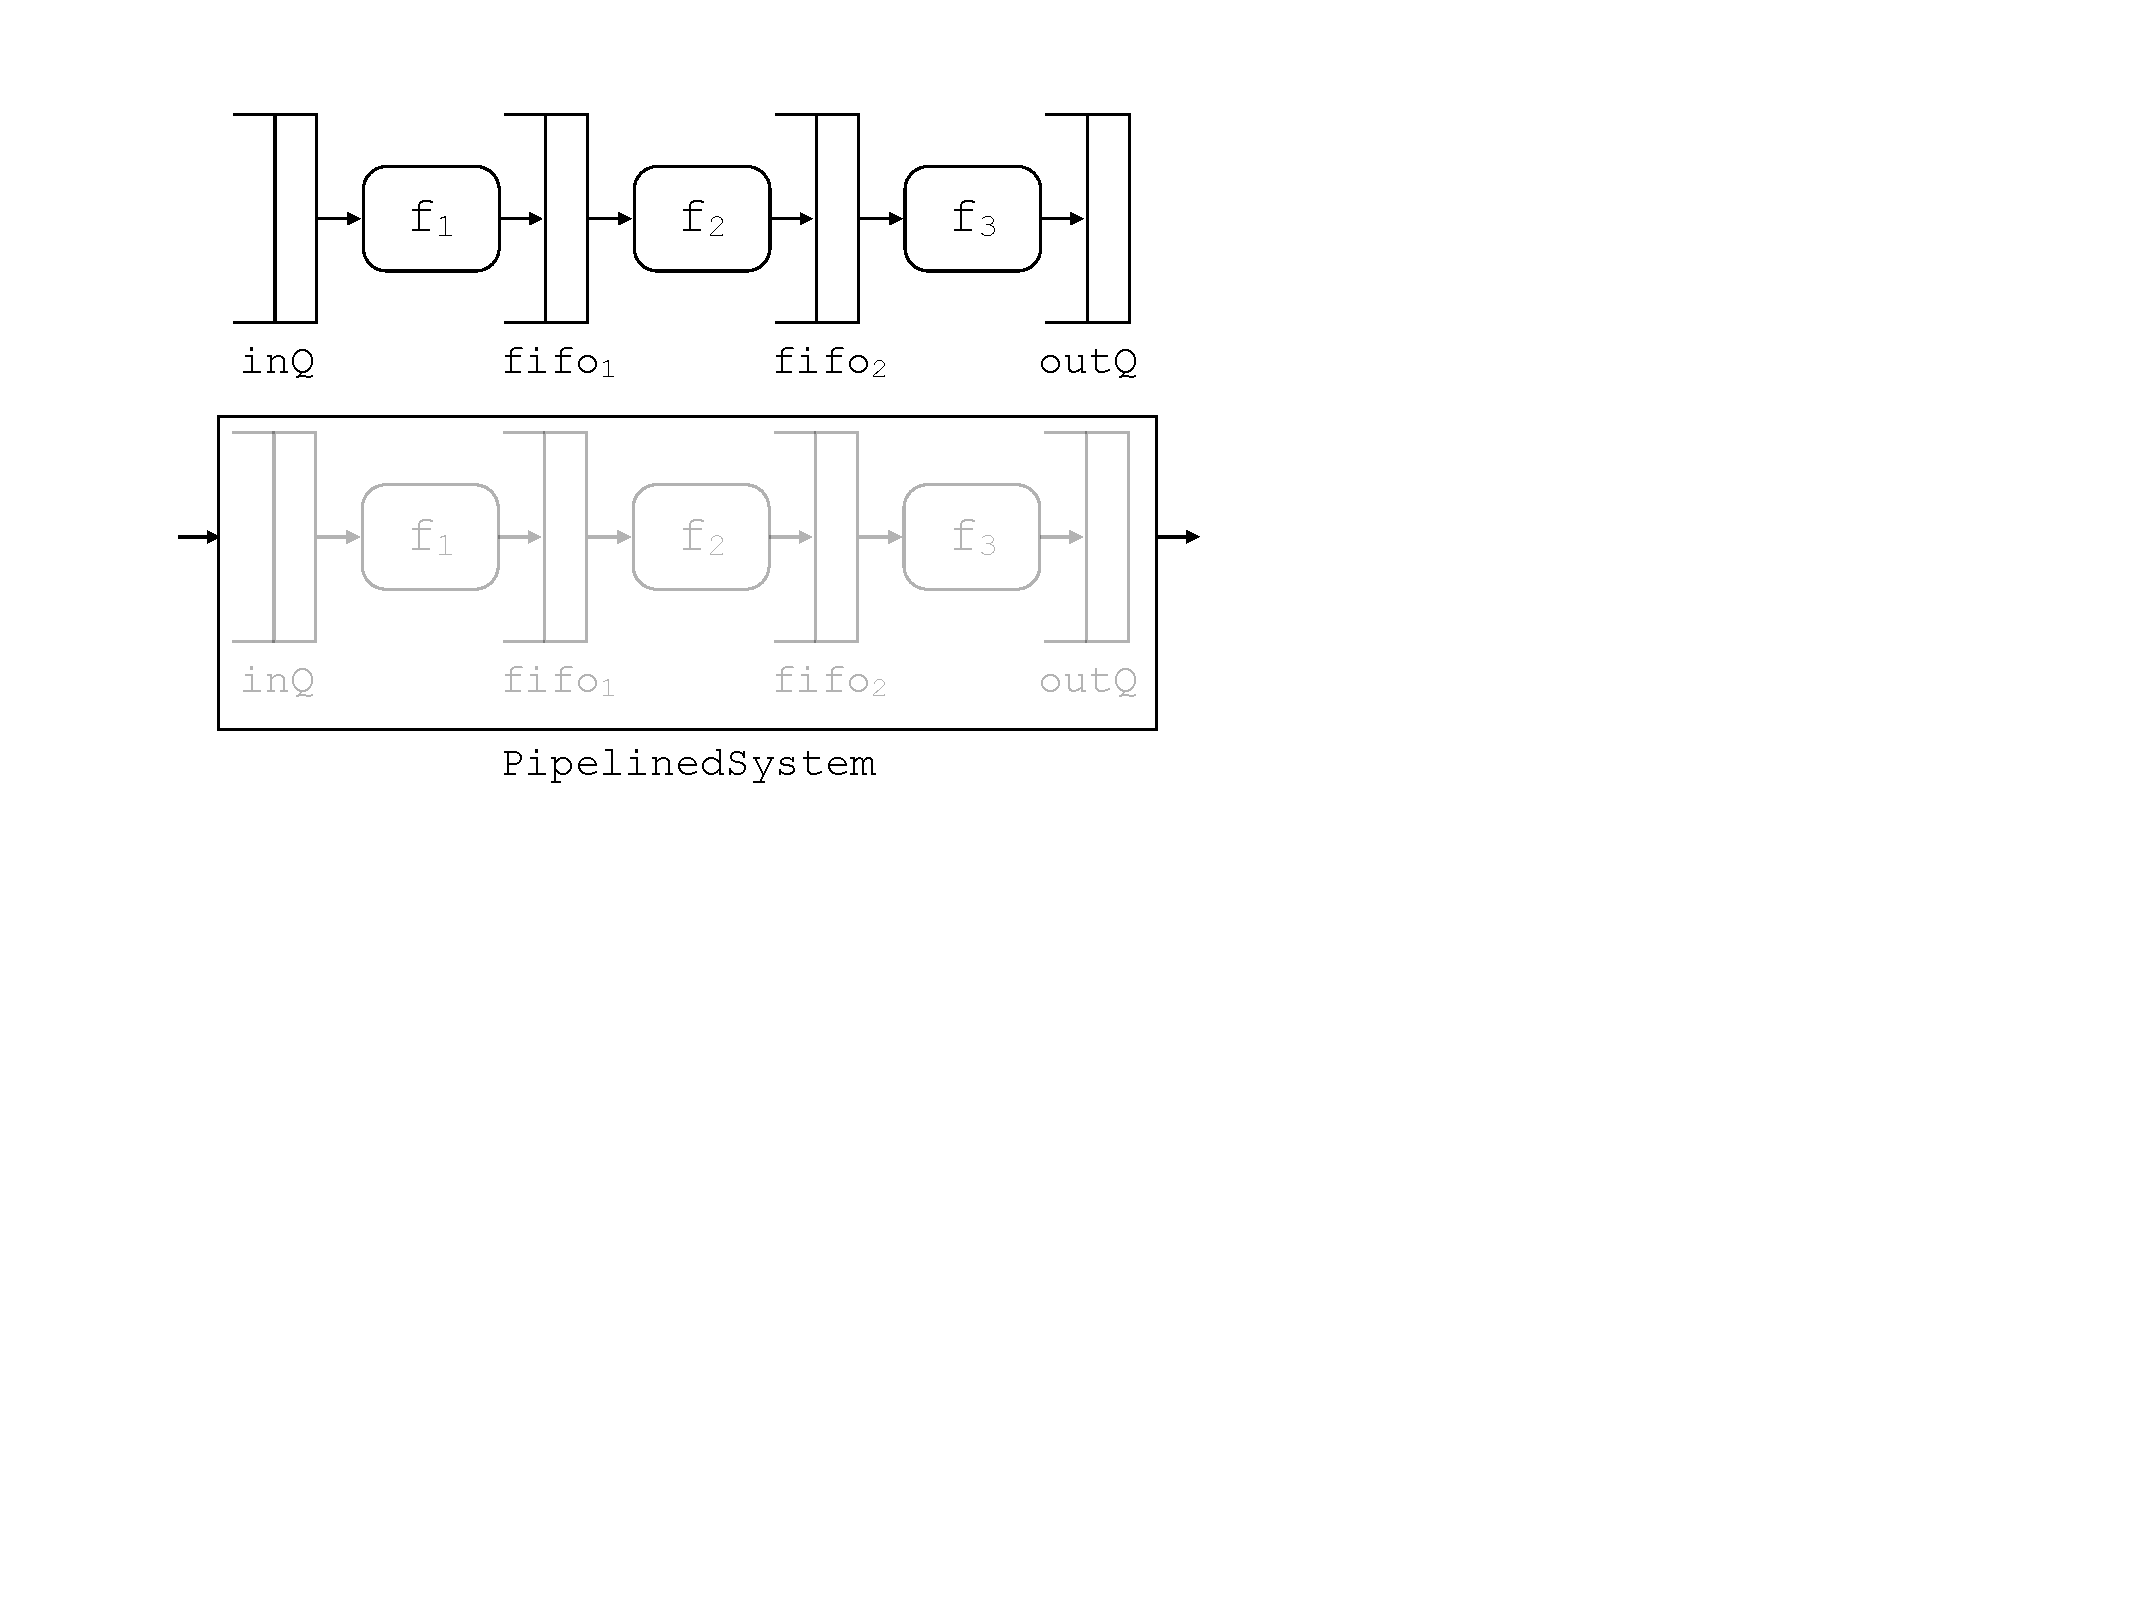
\includegraphics[width=0.6\textwidth]{figures/pipeline-internal.pdf}
  \caption{Internal states hidden by the module}
  \label{ex-modular-semantics-disadvantage}
\end{figure}

However, the modular semantics has an inherent weakness that it is
hard to track internal state changes by internal communications.
Suppose we designed a pipelined system, as shown in the upper part of
\reffig{ex-modular-semantics-disadvantage}. $\texttt{f}_1$,
$\texttt{f}_2$, and $\texttt{f}_3$ are modules which get an input from
the corresponding fifos $\texttt{inQ}$, $\texttt{fifo}_1$, and
$\texttt{fifo}_2$, respectively. When the system is built, modular
semantics abstract the system as a big module, in which only two
interfaces are revealed: one for input to $\texttt{inQ}$, and the
other for output from $\texttt{outQ}$ (as shown in the lower part of
the figure where internal modules are drawn vaguely). In this case,
when having information for an input and the output by the entire
system, how can we describe the \emph{internal state changes} in the
system? For instance, is $\texttt{fifo}_1$ storing an element for
given input and output? In modular semantics, we even cannot draw the
fact that the system is implemented by pipelines, since the semantics
are not defined by following execution paths, but by a series of local
communication among small modules.

A number of semantics, which do not have such a weakness, have been
defined but none of them was defined for open systems. In other words,
there have been no semantics which is able to define communication
with external modules. A big-step semantics along with the action
structures in \Bluespec{} have been defined~\cite{nirav-memocode}, but
it does not have a notion for external communications.

Hence, in this thesis, I present an additional semantics definition,
which is based on inlining.  The inlining semantics is defined for
open hardware systems and resolve the weakness by construction.  The
semantics use a static inlining operation to substitute internal calls
to their method bodies. This operator erases all internal calls in a
module, so that we do not need to care about internal communications.

An implication from the modular semantics to the inlining semantics is
also formally proven, thus it can be used to handle the semantics
efficiently. Since the two semantics does not have equal capabilities,
we give the implication proof saying that the modular semantics imply
the inlining semantics.

To sum up, the main contributions of this thesis are:
\begin{itemize}
\item To define a new semantics definition based on inlining, for open
  hardware systems.
\item To prove the implication from the modular semantics to the
  inlining semantics.
\end{itemize}

\paragraph{Overview}

The thesis is organized as follows: \refchap{chap:backgrounds}
explains a number of prerequisites to understand the hardware design
concept of \Bluespec{}. Related works are also provided to compare
previous approaches to define hardware
semantics. \refchap{chap:semantics} presents the two semantics used in
the \Kami{} framework: modular and inlining
semantics. \refchap{chap:implication} compares capability of each
semantics and presents the implication proof between
semantics. Lastly, we draw conclusions and give future works in
\refchap{chap:conclusions}.





